\documentclass[11pt,a4paper]{article}
\usepackage[utf8]{inputenc}
\usepackage[T1]{fontenc}
\usepackage[spanish,es-nodecimaldot]{babel}
\usepackage[margin=2.5cm]{geometry}
\usepackage{amsmath,amssymb,booktabs,longtable,array}
\usepackage{graphicx}\graphicspath{{muografia-documentada/objetivo-1/figuras/cierre-2026-10-03/}{../figuras/cierre-2026-10-03/}{objetivo-1/figuras/cierre-2026-10-03/}}
\usepackage{hyperref}
\hypersetup{colorlinks=true,linkcolor=blue,urlcolor=blue,citecolor=blue}
\setlength{\parskip}{0.45em}
\setlength{\parindent}{1.2em}
\setlength{\emergencystretch}{2em}
\newcommand{\E}{\mathbb{E}}
\newcommand{\Var}{\operatorname{Var}}
\newcommand{\Cov}{\operatorname{Cov}}
\newcommand{\ind}{\mathbf{1}}
\title{Generación y verificación del conjunto sintético de muografía\\Informe de cierre del objetivo específico 1}
\author{}
\date{3 de octubre de 2026}
\begin{document}
\maketitle

\noindent\textbf{Estado del documento.} Informe de cierre del OE1 bajo el alcance idealizado adoptado por la dirección. El 3 de octubre de 2026 se solicitó expresamente consolidar y cerrar este objetivo con la evidencia disponible. Se integran la metodología, la justificación de representatividad, los resultados, las figuras y la conclusión de cumplimiento. La ejecución en SC3 corresponde a los estudiantes; la revisión local y la consolidación documental corresponden al seguimiento de la dirección. Este cierre no constituye aprobación institucional de la tesis ni validación de un detector real.

\begingroup\small\tableofcontents\endgroup\clearpage

\section{Alcance y nomenclatura}

El objetivo específico 1 del plan aprobado (sección 4.2, página 9) establece:
\begin{quote}
Generar un conjunto de datos sintéticos de imágenes muográficas por transmisión, con diferentes niveles de estadística de conteo, mediante simulación Monte Carlo que reproduzca escenarios representativos de exploración volcánica.
\end{quote}

El objetivo de esta etapa consistió en obtener un conjunto de imágenes sintéticas de muografía por transmisión que representara escenarios volcánicos idealizados y diferentes niveles de estadística de conteo. Para ello se articuló la definición de geometrías con el transporte Monte Carlo de muones, la formación de histogramas angulares y la construcción de realizaciones de menor conteo. El producto permite estudiar variaciones estadísticas sobre una familia controlada de escenarios; su alcance no comprende la reproducción de un volcán particular ni la respuesta completa de un instrumento de campo.

Conviene distinguir tres unidades del conjunto. Una \emph{geometría} especifica el edificio y sus heterogeneidades internas. Una \emph{vista} fija la posición o dirección nominal desde la que se observa esa geometría. Una \emph{realización de menor conteo} se obtiene estadísticamente a partir de la imagen de referencia de una vista. Así, cambiar la realización no equivale a cambiar la geometría ni a ejecutar una nueva simulación de transporte.

Se adopta la nomenclatura de la tabla siguiente. Los índices de píxel y de vista comienzan en cero para conservar la correspondencia con los archivos. Las cantidades sin unidades explícitas son adimensionales o conteos, según su definición.

\begingroup\small\begin{longtable}{p{0.22\textwidth}p{0.70\textwidth}}
\toprule Símbolo & Definición y correspondencia \\ \midrule
\endhead
$g$, $v$ & Identificador de geometría y vista $v\in\{0,\ldots,5\}$. \\
$i$, $j$ & Fila de elevación y columna de azimut, respectivamente; $i,j\in\{0,\ldots,255\}$. \\
$\varphi$, $\eta$ & Azimut relativo a la vista y elevación sobre el horizonte, expresados en grados. \\
$N_{gv}$ & Número de primarios transportados en una vista; campo \texttt{events\_transported}. \\
$N^{\mathrm{nom}}_{gv}$ & Primarios generados dentro de la ventana nominal; campo \texttt{nominal\_in\_window}. \\
$C_{gvij}$ & Conteo de referencia del píxel $(i,j)$; arreglo \texttt{counts\_ref}. \\
$D_{gv}$ & Suma de los conteos de referencia de una vista; campo \texttt{detected\_in\_bins}. \\
$f$, $k$ & Fracción de adelgazamiento y realización $k\in\{0,\ldots,19\}$. \\
$L^{(f,k)}_{gvij}$ & Conteo reducido; arreglo \texttt{low\_counts}, indexado por fracción, realización, fila y columna. \\
$\rho_g(\boldsymbol{x})$ & Densidad de masa de la geometría, en $\mathrm{g\,cm^{-3}}$. \\
$X_g(\ell)$ & Columna de masa sobre una trayectoria $\ell$, en $\mathrm{g\,cm^{-2}}$. \\
$r$, $r_0$ & Región angular de control e interior utilizado como referencia del contraste de bordes. \\
$K_{gvr}$ & Conteo agregado de la región $r$. \\
$p^{\mathrm{nom}}_r$, $p^{\mathrm{ideal}}_r$ & Probabilidades tabuladas, por primario generado, para la región y la selección ideal. \\
$e_{gvr}$, $d_{gvr}$ & Residuo normalizado y diferencia de ese residuo respecto al interior. \\
$Q_{gvq}$, $F_{gv}$ & Conteo de la ROI $q$ de roca y fracción de ROI de una vista con al menos 100 cuentas. \\
$\alpha$, $\tau$ & Nivel de error familiar y tolerancia del contraste; $\alpha=0.05$, $\tau=0.01$. \\
\bottomrule
\end{longtable}\endgroup

Esta notación reserva $N$ para el presupuesto de transporte y $C$ para las cuentas registradas. Se evita utilizar indistintamente ambas cantidades: una partícula generada puede no llegar al plano, no superar el corte energético o quedar fuera de la ventana angular de registro. Asimismo, $X$ denota columna de masa y no intensidad de imagen.

\section{Metodología de generación y preparación}
\label{sec:metodologia}

\subsection{Escenarios geométricos y sentido de las imágenes}

El catálogo contiene 19 geometrías cónicas: 18 incorporan anomalías internas y una representa un edificio homogéneo. Cada escenario se observa desde seis vistas con separación nominal de $60^\circ$, para un total de 114 combinaciones geometría--vista. El catálogo permite variar características geométricas y contrastes de densidad manteniendo una representación simplificada del edificio. No constituye una muestra de 19 volcanes medidos ni de 19 orientaciones de un mismo modelo.

Para describir matemáticamente la idealización, un cono recto de radio basal $R_g$ y altura $H_g$, referido a una base horizontal en $z=0$, puede expresarse como
\begin{equation}
 \mathcal V_g=\left\{(x,y,z):0\leq z\leq H_g,\quad
 \sqrt{x^2+y^2}\leq R_g\left(1-\frac{z}{H_g}\right)\right\}.
\end{equation}
Esta expresión fija el significado geométrico de radio y altura; la ubicación efectiva, los materiales y las anomalías se especifican en los archivos de cada escenario. Los conductos y cuerpos internos modifican la distribución de masa encontrada por las trayectorias. La columna de masa se define por
\begin{equation}
 X_g(\ell)=\int_{\ell\cap\mathcal V_g}\rho_g(\boldsymbol{x})\,\mathrm ds,
 \qquad [X_g]=\mathrm{g\,cm^{-2}},
 \label{eq:columna}
\end{equation}
si la longitud se expresa en centímetros. Esta magnitud describe la masa por unidad de área atravesada a lo largo del camino considerado. No se identifica directamente con el valor de un píxel: la cuenta observada depende también de la distribución de energía y dirección de los muones, de su transporte y de la regla de selección.

Por ejemplo, el catálogo de \texttt{geo-train-06} establece un radio basal de $509.7\,\mathrm m$, una altura de $416.3\,\mathrm m$ y una densidad de roca de $2.65\,\mathrm{g\,cm^{-3}}$. Incluye un conducto de radio $21.0\,\mathrm m$ y densidad $1.832\,\mathrm{g\,cm^{-3}}$, además de un cuerpo denso elipsoidal de $3.285\,\mathrm{g\,cm^{-3}}$. Estos valores ilustran la parametrización de un escenario y no deben extenderse a todo el catálogo. La configuración y sus huellas, no una figura esquemática, identifican el modelo utilizado.

\subsection{Justificación de la representatividad dentro del alcance adoptado}

La representatividad del conjunto se entiende como cobertura de mecanismos y configuraciones de contraste relevantes para un estudio sintético de transmisión, y no como representatividad estadística de una población de volcanes reales. Esta distinción relaciona el objetivo aprobado con el producto efectivamente generado: se seleccionan situaciones que permiten examinar variaciones de trayectoria, columna de masa y conteo bajo condiciones controladas.

El catálogo verificado abarca radios basales de $509.7$ a $698.7\,\mathrm m$ y alturas de $356.2$ a $449.6\,\mathrm m$, con roca de fondo de $2.65\,\mathrm{g\,cm^{-3}}$. Incluye conductos de menor densidad, cavidades y cuerpos de mayor densidad, tanto aislados como combinados. Las cavidades son regiones de baja densidad asignada; no se presupone vacío perfecto. Esta construcción permite contrastar un fondo homogéneo con déficits y excesos de masa, y examinar cómo cambia su proyección al variar la vista. Los intervalos describen el catálogo, no rangos validados de una población geológica.

La geometría homogénea es \texttt{geo-train-01}; \texttt{geo-gen-01}, reservada para generalización, contiene un conducto y dos cavidades. Se conserva esta identificación para evitar atribuir al caso reservado una condición de control homogéneo que no posee. Las diecinueve huellas de geometría coinciden con las registradas en la receta de producción.

La pertinencia de las anomalías se interpreta a través de la columna de masa de la ecuación~\eqref{eq:columna}. Para un camino fijo y una región de longitud $\ell_a$ en la que se sustituye la densidad de fondo $\rho_0$ por $\rho_a$, el cambio nominal es
\begin{equation}
 \Delta X=(\rho_a-\rho_0)\ell_a.
\end{equation}
Con longitud en centímetros, $\Delta X$ queda en $\mathrm{g\,cm^{-2}}$. Su signo distingue déficits y excesos de masa; no convierte el conteo en una medición directa de densidad ni impone una relación lineal entre $\Delta X$ y la imagen. En el transporte intervienen además energía, dispersión y selección de llegada. La expresión justifica la diversidad de contrastes elegida, sin sustituir el cálculo Monte Carlo.

\begin{center}
\begin{tabular}{p{0.24\textwidth}p{0.33\textwidth}p{0.32\textwidth}}
\toprule Componente & Papel en el diseño & Límite de interpretación\\\midrule
Edificios cónicos y dimensiones variables & Variación controlada de caminos y columnas de masa. & No reproduce topografía ni estratigrafía de un volcán particular.\\
Fondo homogéneo & Caso sin anomalías del catálogo. & No es una referencia de cielo abierto.\\
Conductos y cavidades & Configuraciones de déficit de densidad. & No identifica composición ni estado geológico real.\\
Cuerpos densos y combinaciones & Contrastes positivos y coexistencia de heterogeneidades. & No demuestra detectabilidad o separación de anomalías.\\
Seis vistas por escenario & Cambio de proyección con la dirección de observación. & No son seis edificios independientes.\\
Cuatro fracciones de conteo & Degradación estadística controlada. & No calibra exposición física del instrumento.\\\bottomrule
\end{tabular}
\end{center}

La fuente tabulada, el transporte de primarios y el plano computacional fijan un mismo problema de generación para todas las vistas. Esa consistencia permite interpretar diferencias dentro del conjunto. La suficiencia de esta representatividad para el OE1 se acepta bajo el alcance idealizado adoptado por la dirección; no se extrapola a equivalencia experimental. Las limitaciones permanecen como parte de la conclusión y no como pruebas supuestamente realizadas.

\subsection{Fuente de muones y configuración de transporte}

La cadena utiliza Geant4 como infraestructura de transporte de partículas \cite{agostinelli2003}. En la campaña se registró Geant4 11.4.2 con la lista de física FTFP\_BERT y una configuración que conserva únicamente primarios. Por tanto, la lista de física utilizada no debe interpretarse como evidencia de que el conjunto incluya todas las contribuciones secundarias o el fondo de un detector real.

La fuente efectiva es híbrida. Emplea pesos angulares derivados de la parametrización de Guan y colaboradores \cite{guan2015}, y tablas de cuantiles de momento obtenidas a partir de EcoMug \cite{pagano2021}. Esta descripción es más precisa que atribuir a EcoMug la generación directa de cada evento durante la campaña: el procedimiento de producción utiliza tablas y reglas de interpolación propias, registradas en la receta del proyecto \cite{receta}.

Los puntos de impacto nominal se muestrean uniformemente sobre un panel cuadrado de $1.2\,\mathrm m$ de lado. El azimut de generación se extiende entre $-35^\circ$ y $35^\circ$ respecto de la vista, mientras que la ventana nominal de imagen abarca $-30^\circ$ a $30^\circ$. El margen angular de $5^\circ$ incorpora direcciones adicionales a la ventana de registro. En elevación se conservan los pesos tabulados en el intervalo nominal y se utiliza la extensión documentada en los extremos; los pesos negativos y los centros por debajo de $0.1^\circ$ se anulan. El momento se obtiene mediante interpolación lineal por tramos de 257 cuantiles en 16 bandas de elevación, utilizando la banda extrema más cercana fuera del dominio tabulado.

La inyección se establece cerca del edificio mediante un recorrido inverso de la trayectoria nominal, con muestreo espacial cada $0.5\,\mathrm m$ hasta $4\,\mathrm{km}$ y un desplazamiento adicional de $1\,\mathrm m$ respecto al último punto interior identificado. Cuando no se identifica intersección, se aplica la regla de inyección previa al panel descrita en la receta. Se trata de una construcción numérica de la fuente, cuya interpretación está ligada al alcance idealizado adoptado.

El plano de registro tiene $600\,\mathrm m$ de lado. Su función es computacional: permite contar cruces y analizar direcciones después del transporte. No equivale al panel nominal de $1.2\,\mathrm m$ ni acredita la aceptación de un instrumento real de ese tamaño. Para contribuir al histograma, un muon primario debe satisfacer el criterio de cruce, pertenecer a la ventana angular y conservar energía cinética superior a $3\,\mathrm{GeV}$ en el plano. El umbral se aplica a la energía cinética al registrar la llegada, no a una etiqueta de exposición ni, por identidad, al momento inicial.

\subsection{Presupuesto, bloques y formación de la referencia}

Se fijó un presupuesto de
\begin{equation}
 N_{gv}=344\times10^6,\qquad
 N_{\mathrm{camp}}=\sum_g\sum_{v=0}^{5}N_{gv}
 =19\times6\times344\times10^6
 =39\,216\,000\,000.
 \label{eq:presupuesto}
\end{equation}
Cada vista se distribuyó en nueve bloques identificados mediante semillas y registros de ejecución, con 1.026 bloques en total. La consolidación suma los conteos de los bloques aceptados de una misma vista, sin duplicar reintentos. Si $C^{[b]}_{gvij}$ es el conteo del bloque $b$, la referencia se obtiene como
\begin{equation}
 C_{gvij}=\sum_{b=1}^{9}C^{[b]}_{gvij},\qquad
 D_{gv}=\sum_{i=0}^{255}\sum_{j=0}^{255}C_{gvij}\leq N_{gv}.
 \label{eq:conteos}
\end{equation}
La desigualdad corresponde al contrato de, como máximo, un registro por primario. Los conteos se almacenan como enteros sin signo de 32 bits, sin suavizado ni recorte de amplitud.

Una representación equivalente del píxel es
\begin{equation}
 C_{gvij}=\sum_{n=1}^{N_{gv}}\ind\{A_{gvn},\;E^{\mathrm{kin}}_{gvn}>3\,\mathrm{GeV},
 \;(\eta_{gvn},\varphi_{gvn})\in B_{ij}\},
 \label{eq:indicador}
\end{equation}
donde $A_{gvn}$ denota un cruce primario aceptado, $E^{\mathrm{kin}}_{gvn}$ su energía cinética al llegar al plano y $B_{ij}$ el intervalo angular del píxel. Las direcciones son las registradas después del transporte. La ecuación deja explícito que la imagen representa cuentas direccionales; no es una fotografía del edificio, un mapa de densidad ni una matriz de transmisión física ya calibrada.

\subsection{Malla angular y correspondencia de índices}

La matriz tiene 256 filas de elevación y 256 columnas de azimut. La convención \texttt{az-edges-v1} fija los bordes azimutales como
\begin{equation}
 \varphi^{\mathrm e}_j=-30^\circ+j\frac{60^\circ}{256},\quad j=0,\ldots,256,
 \qquad \varphi_j=\frac{\varphi^{\mathrm e}_j+\varphi^{\mathrm e}_{j+1}}{2}.
\end{equation}
La separación es $0.234375^\circ$ y el primer centro se encuentra en $-29.8828125^\circ$. En elevación, la convención conservada especifica centros, no bordes:
\begin{equation}
 \eta_i=2^\circ+i\frac{45^\circ}{255},\quad i=0,\ldots,255,
 \qquad \Delta\eta=\frac{45^\circ}{255}.
\end{equation}
Los bordes se obtienen de los puntos medios entre centros, extendiendo medio paso en ambos extremos. En consecuencia, el soporte nominal de los intervalos de elevación es aproximadamente $[1.911765^\circ,47.088235^\circ]$. Describirlo simplemente como bordes entre $2^\circ$ y $47^\circ$ introduciría una discrepancia de medio píxel con los archivos.

Se conservan los centros y bordes en los arreglos \texttt{az\_\allowbreak centers\_\allowbreak deg}, \texttt{az\_\allowbreak edges\_\allowbreak deg}, \texttt{el\_\allowbreak centers\_\allowbreak deg} y \texttt{el\_\allowbreak edges\_\allowbreak deg}. Si se utiliza el ángulo cenital en una discusión de la fuente, deberá distinguirse de la elevación: para una misma dirección referida al horizonte y a la vertical, la conversión es $\theta=90^\circ-\eta$. No se sustituye una variable por otra sin efectuar esa conversión.

\subsection{Adelgazamiento binomial y construcción de pares}

Para cada referencia se consideraron las fracciones
\begin{equation}
 \mathcal F=\{0.50,0.10,0.05,0.01\},\qquad k=0,\ldots,19.
\end{equation}
El conteo reducido se generó mediante
\begin{equation}
 L^{(f,k)}_{gvij}\mid C_{gvij}=c\;\sim\;\operatorname{Binomial}(c,f).
 \label{eq:binomial}
\end{equation}
Cada cuenta de la referencia tiene probabilidad $f$ de ser conservada. La operación produce enteros entre cero y $c$, sin añadir conteos nuevos. Las veinte realizaciones se generan con flujos pseudoaleatorios separados para cada geometría, vista y fracción. La semilla maestra es 20260805 y la derivación combina el identificador de geometría, la vista, el índice de fracción y el de realización, según el esquema registrado en el empaquetador \cite{datos}.

De la distribución condicional se obtienen
\begin{align}
 \E[L^{(f,k)}_{gvij}\mid C_{gvij}]&=fC_{gvij},\\
 \Var(L^{(f,k)}_{gvij}\mid C_{gvij})&=f(1-f)C_{gvij}.
 \label{eq:momentos}
\end{align}
Por ello, reducir el conteo no consiste en multiplicar la imagen por $f$: esa multiplicación solo reproduce la media condicional y omite la fluctuación estadística que se pretende representar. El par se define como la matriz reducida y su referencia,
\begin{equation}
 \mathcal P_{gvfk}=\left(\boldsymbol L^{(f,k)}_{gv},\boldsymbol C_{gv}\right),
 \qquad n_{\mathrm{pares}}=19\times6\times4\times20=9\,120.
\end{equation}
El archivo conserva las cuentas originales; no almacena, como sustituto de ellas, $L/f$. Si posteriormente se utiliza ese reescalamiento para una comparación, debe declararse como una transformación adicional.

La referencia de alta estadística también es aleatoria. Bajo un modelo de historias independientes con presupuesto fijo, un píxel con probabilidad de registro $\pi_{gvij}$ satisface $C_{gvij}\sim\operatorname{Binomial}(N_{gv},\pi_{gvij})$. En ese modelo, el adelgazamiento produce marginalmente $L^{(f,k)}_{gvij}\sim\operatorname{Binomial}(N_{gv},f\pi_{gvij})$. Esto no es idéntico, para presupuesto fijo, a transportar exactamente $fN_{gv}$ historias con probabilidad $\pi_{gvij}$; las medias coinciden pero las varianzas no son, en general, iguales. La interpretación de menor exposición es estadística y depende del modelo de adquisición que se adopte.

Además, aunque los sorteos de realizaciones distintas sean condicionalmente independientes dada la referencia, comparten su fluctuación. Para un mismo píxel y dos sorteos distintos $a$ y $b$, con fracciones $f_a$ y $f_b$, las identidades de esperanza y covarianza condicional dan
\begin{align}
 \Cov(L^{a},C)&=f_a\Var(C),\\
 \Cov(L^{a},L^{b})&=f_af_b\Var(C).
 \label{eq:dependencia}
\end{align}
Se suprimieron los índices del píxel solo en estas dos expresiones. Las ecuaciones explican por qué los 80 pares de una vista no representan 80 referencias de transporte independientes. También justifican mantener juntas las realizaciones procedentes de una misma geometría al particionar el conjunto.

\subsection{Particiones y exposición convencional}

La separación se realiza por geometría, conservando todas las vistas, fracciones y realizaciones del escenario en una misma partición. Se asignaron 12 geometrías a entrenamiento, tres a validación, tres a prueba y una a generalización. En términos de geometrías, esto representa aproximadamente $63.16\%$, $15.79\%$, $15.79\%$ y $5.26\%$, respectivamente. Se informa la asignación efectiva; no se la presenta como una división aleatoria de los 9.120 pares.

\begin{center}
\begin{tabular}{lrrr}
\toprule Partición & Geometrías & Referencias & Pares\\\midrule
Entrenamiento &12&72&5\,760\\
Validación &3&18&1\,440\\
Prueba &3&18&1\,440\\
Generalización &1&6&480\\\midrule
Total &19&114&9\,120\\\bottomrule
\end{tabular}
\end{center}

El presupuesto de simulación es un número de primarios y no una duración física. El campo \texttt{exposure\_days} toma el valor $-1$, que identifica la modalidad de presupuesto fijo y no un tiempo negativo. Se conserva, por separado, la etiqueta
\begin{equation}
 T^{\mathrm{conv}}_{gv}=30\,\mathrm{d}_{\mathrm{conv}}
 \frac{N^{\mathrm{nom}}_{gv}}{S_0},\qquad
 S_0=36\,034\,069.911914065.
 \label{eq:exposicion}
\end{equation}
Aquí $\mathrm{d}_{\mathrm{conv}}$ designa la unidad convencional usada en los metadatos y $S_0$ es el conteo de referencia de esa escala. El numerador cuenta generación nominal, no llegadas detectadas. Sin una calibración de flujo, aceptación y respuesta instrumental, esta expresión no establece cuántos días mediría un detector real. Tampoco permite inferir directamente una reducción de tiempo de adquisición a partir de las fracciones de adelgazamiento.

\section{Procedimiento de verificación}

\subsection{Integridad, procedencia y reproducción del posproceso}

La verificación siguió la cadena de procedencia desde los histogramas consolidados hasta las referencias y los pares. Se compararon huellas SHA-256, se comprobó la identidad de conteos y coordenadas entre CSV y NPZ, y se reprodujo la evaluación desde los píxeles. Posteriormente se regeneraron los pares con NumPy 2.4.4 y se compararon sus arreglos contra las huellas publicadas. Esta reproducción corresponde al posproceso; no constituye una segunda ejecución local de Geant4.

Para la copia distribuida en Drive se distinguió entre integridad del archivo e identidad numérica. La huella de un NPZ depende de sus bytes comprimidos, que pueden cambiar con la versión de compresión. La huella de contenido utilizada en esta revisión concatena la representación del tipo, la forma y los bytes contiguos del arreglo en orden C antes de aplicar SHA-256. De este modo se comprueba que la regeneración conserva los valores, dimensiones y tipos, además de validar los archivos contra el manifiesto de su propia copia \cite{drive}.

\subsection{Contraste de bordes respecto a una fuente ideal}

El control de bordes no exige que todos los píxeles tengan la misma cuenta. El espectro y los pesos angulares varían con la elevación; por ello, el contraste compara la respuesta con una referencia tabulada compatible con la fuente. Se definieron quince regiones de borde por vista: cinco columnas de cada extremo azimutal, restringidas al cielo entre $30^\circ$ y $42^\circ$ de elevación, y las cinco filas superiores. Se añadió una región interior de cielo en el mismo intervalo de elevación, excluyendo veinte columnas por cada lado. Las máscaras se conservan con sus huellas en el plan de campaña.

El conteo agregado de una región es $K_{gvr}=\sum_{(i,j)\in r}C_{gvij}$. El residuo adoptado en el evaluador se expresa como
\begin{equation}
 e_{gvr}=\frac{K_{gvr}/N_{gv}-p^{\mathrm{ideal}}_r}{p^{\mathrm{nom}}_r},
 \qquad d_{gvr}=e_{gvr}-e_{gvr_0}.
 \label{eq:residuo}
\end{equation}
Las dos probabilidades de referencia se tratan como cantidades fijas tabuladas. La primera resta ajusta la selección ideal correspondiente a la región, mientras que la división expresa el residuo por probabilidad de inyección nominal. El contraste con el interior examina una diferencia de respuesta bajo esa definición; no estima por sí solo transmisión instrumental calibrada ni identifica la causa de una discrepancia.

Con historias independientes y máximo un registro por primario, $K_{gvr}$ tiene una distribución binomial marginal con $N_{gv}$ ensayos. Para acotar sus probabilidades se emplearon intervalos Clopper--Pearson, implementados mediante cuantiles beta en el evaluador del proyecto \cite{estadistica}. Para $K=K_{gvr}$, $N=N_{gv}$ y
\begin{equation}
 \alpha_* = \frac{0.05}{114\times16},
\end{equation}
los límites son
\begin{align}
 a_r&=\begin{cases}0,&K=0,\\
 B^{-1}(\alpha_*/2;K,N-K+1),&K>0,\end{cases}\\
 b_r&=\begin{cases}1,&K=N,\\
 B^{-1}(1-\alpha_*/2;K+1,N-K),&K<N,\end{cases}
\end{align}
donde $B^{-1}(u;a,b)$ es el cuantil $u$ de una distribución beta de parámetros $a,b$. El factor 16 incluye las quince regiones de borde y el interior; el factor 114 incorpora todas las vistas. La corrección de Bonferroni proporciona cobertura simultánea de al menos $95\%$ bajo el modelo indicado, sin exigir independencia entre las regiones.

Al transformar los extremos según la ecuación~\eqref{eq:residuo}, se obtiene un intervalo $[e^-_{gvr},e^+_{gvr}]$ para cada residuo. El intervalo conservador del contraste es
\begin{equation}
 I_{gvr}=\left[e^-_{gvr}-e^+_{gvr_0},\;
 e^+_{gvr}-e^-_{gvr_0}\right].
\end{equation}
Se declara conformidad únicamente si $I_{gvr}\subseteq[-0.01,0.01]$. En la presentación de resultados se multiplica por 100, de modo que la tolerancia es de $\pm1$ punto porcentual en la escala normalizada definida. No basta que el estimador puntual esté dentro del intervalo de tolerancia. La cobertura estadística tampoco incluye incertidumbre de las hipótesis físicas de la referencia ideal.

\subsection{Estadística de conteo en roca}

Para describir la suficiencia estadística se agruparon píxeles contiguos en ROI de $4\times4$. La selección espacial utiliza la columna nominal del cono homogéneo entre $30\,000$ y $100\,000\,\mathrm{g\,cm^{-2}}$. Esta máscara caracteriza una región específica de roca: no abarca toda la imagen ni incorpora las anomalías en su criterio de selección, aunque las anomalías sí intervienen en el transporte.

Si $\mathcal Q_{gv}$ es el conjunto de ROI seleccionadas, el indicador por vista se define como
\begin{equation}
 Q_{gvq}=\sum_{(i,j)\in q}C_{gvij},\qquad
 F_{gv}=\frac{\sum_{q\in\mathcal Q_{gv}}\ind\{Q_{gvq}\geq100\}}
 {|\mathcal Q_{gv}|}.
 \label{eq:roca}
\end{equation}
La meta descriptiva adoptada fue $F_{gv}\geq0.90$. El umbral de 100 cuentas proporciona una referencia aproximada de fluctuación relativa $1/\sqrt{100}=10\%$ cuando resulta pertinente la aproximación de Poisson. Esa interpretación corresponde a la ROI agregada y al ruido de conteo; no demuestra precisión del $10\%$ por píxel ni incluye el error del modelo físico. La meta de roca y el contraste de bordes responden a preguntas distintas y no deben combinarse en un único criterio sin definición adicional.

\section{Resultados de la campaña y su verificación}

Los registros respaldan la finalización de los 1.026 bloques previstos, correspondientes a las 114 vistas y al presupuesto de la ecuación~\eqref{eq:presupuesto}. La campaña se ejecutó entre el 2 de octubre de 2026 a las 18:10:27 y el 3 de octubre a las 09:48:49, en la partición AMD de SC3. Se solicitaron 64 hilos y $8\,\mathrm{GB}$ por trabajo. Se registraron tres trabajos fallidos que posteriormente se completaron; la consolidación no duplicó los reintentos. La suma de recursos asignados, incluidos los fallos, fue de $2\,356.73$ hilo-horas, magnitud distinta del tiempo transcurrido de reloj y del número de núcleos físicos \cite{campana}.

Se verificaron 248 archivos de fusión y 229 de exportación, para un total de 477 huellas coincidentes con los inventarios. Las 114 matrices exportadas conservaron exactamente las cuentas y coordenadas de los histogramas. La regeneración de los 9.120 pares reprodujo las 342 huellas correspondientes a referencias, conteos reducidos y fracciones de los 114 paquetes. Estos resultados respaldan la trazabilidad y reproducción técnica del conjunto recibido \cite{datos}.

En la comprobación de bordes, los 1.710 intervalos de contraste quedaron completamente dentro de la tolerancia de $\pm1$ punto porcentual. El extremo de mayor valor absoluto fue aproximadamente $0.932696$ puntos porcentuales. Bajo las máscaras, la normalización y el modelo estadístico adoptados, no se identificó un incumplimiento del criterio de bordes. Esta conclusión se limita al contraste definido y no afirma uniformidad absoluta de la imagen ni ausencia de efectos de transporte.

La meta descriptiva de roca se alcanzó en 107 de las 114 vistas. En el conjunto de regiones evaluadas,
\begin{equation}
 F_{\mathrm{global}}=
 \frac{\sum_{g,v}\sum_{q\in\mathcal Q_{gv}}\ind\{Q_{gvq}\geq100\}}
 {\sum_{g,v}|\mathcal Q_{gv}|}
 =\frac{20\,713}{21\,816}\simeq0.949441.
\end{equation}
El $94.944\%$ global pondera las vistas por su número de ROI; no equivale a una media no ponderada de porcentajes ni sustituye la evaluación individual. Las siete vistas bajo la meta se presentan explícitamente para conservar la información de los casos menos favorables.

\begin{center}
\begin{tabular}{lrrrr}
\toprule Geometría & Vista & ROI & ROI con $Q\geq100$ & Porcentaje\\\midrule
\texttt{geo-test-03}&1&222&199&89.640\%\\
\texttt{geo-test-03}&5&222&198&89.189\%\\
\texttt{geo-train-06}&3&244&218&89.344\%\\
\texttt{geo-train-09}&1&206&185&89.806\%\\
\texttt{geo-train-09}&4&206&185&89.806\%\\
\texttt{geo-train-09}&5&206&184&89.320\%\\
\texttt{geo-train-12}&2&234&210&89.744\%\\\bottomrule
\end{tabular}
\end{center}

De acuerdo con el alcance adoptado, estos casos se conservaron sin descartar imágenes, modificar retrospectivamente el umbral ni aumentar automáticamente el presupuesto. Se informa, por tanto, que la campaña alcanzó la meta en la mayoría de las vistas, y no que todas la cumplieron.

La recuperación independiente de Drive produjo 753 archivos y $1\,126\,769\,406$ bytes. Los 2.291 controles de distribución terminaron sin discrepancias: coincidieron las imágenes y los histogramas con Git, los contenidos numéricos de los pares y los manifiestos de la propia copia. También se comprobó la integridad y el contenido del derivado \texttt{dataset-v2}; esta última comprobación no constituye una auditoría del conversor ni una evaluación de aprendizaje profundo \cite{drive}.

\subsection{Visualización de los resultados}

Las figuras~\ref{fig:referencias}--\ref{fig:roca} se generaron desde los datos verificados. Se conservan sus escalas y coordenadas; no se emplearon imágenes ilustrativas como sustituto de resultados.

\begin{figure}[p]\centering
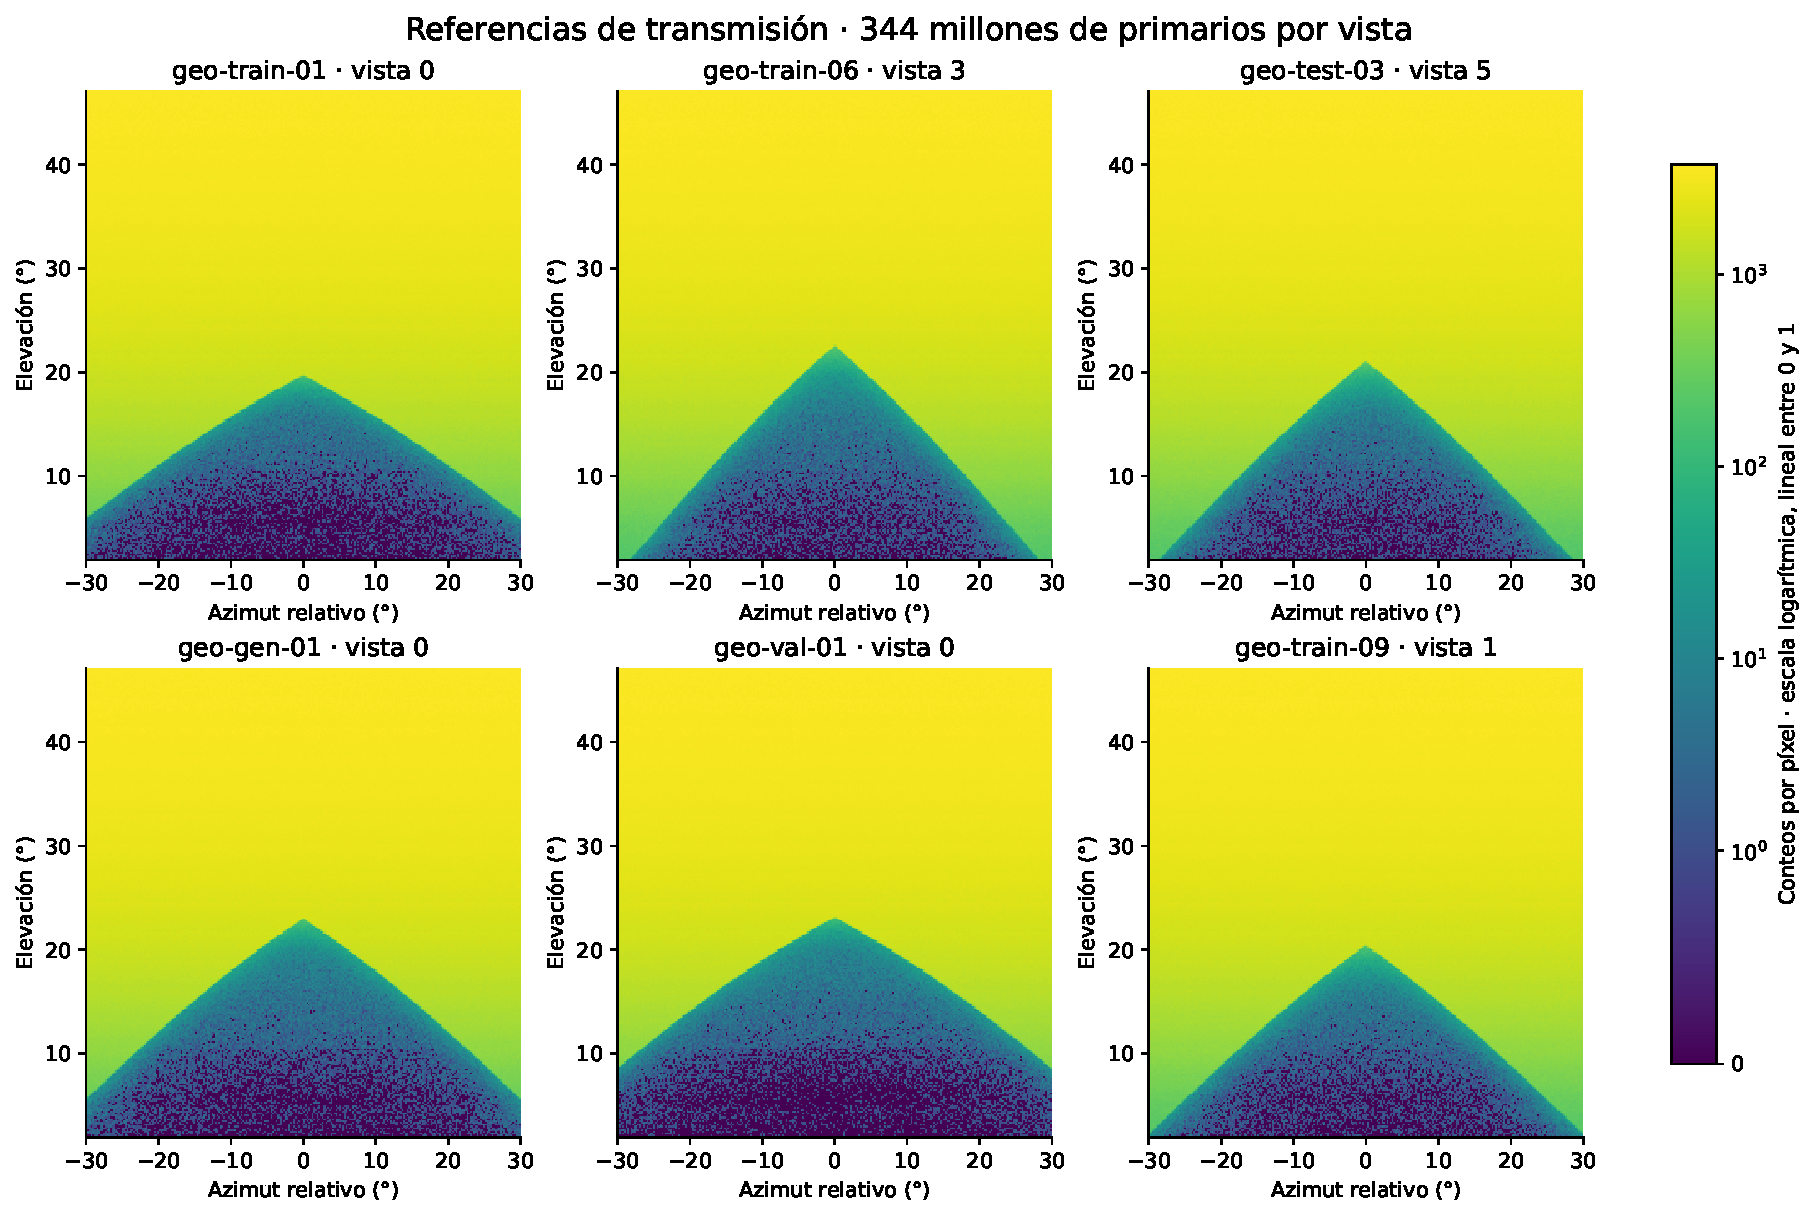
\includegraphics[width=\textwidth]{01-referencias.pdf}
\caption{Referencias de distintas geometrías y vistas. Seis ejemplos con conteos por píxel y coordenadas angulares, sin suavizado. La escala común es logarítmica y lineal entre cero y una cuenta. Incluyen casos bajo la meta de roca; no son una muestra estadística representativa ni mapas de densidad.}\label{fig:referencias}
\end{figure}
\begin{figure}[p]\centering
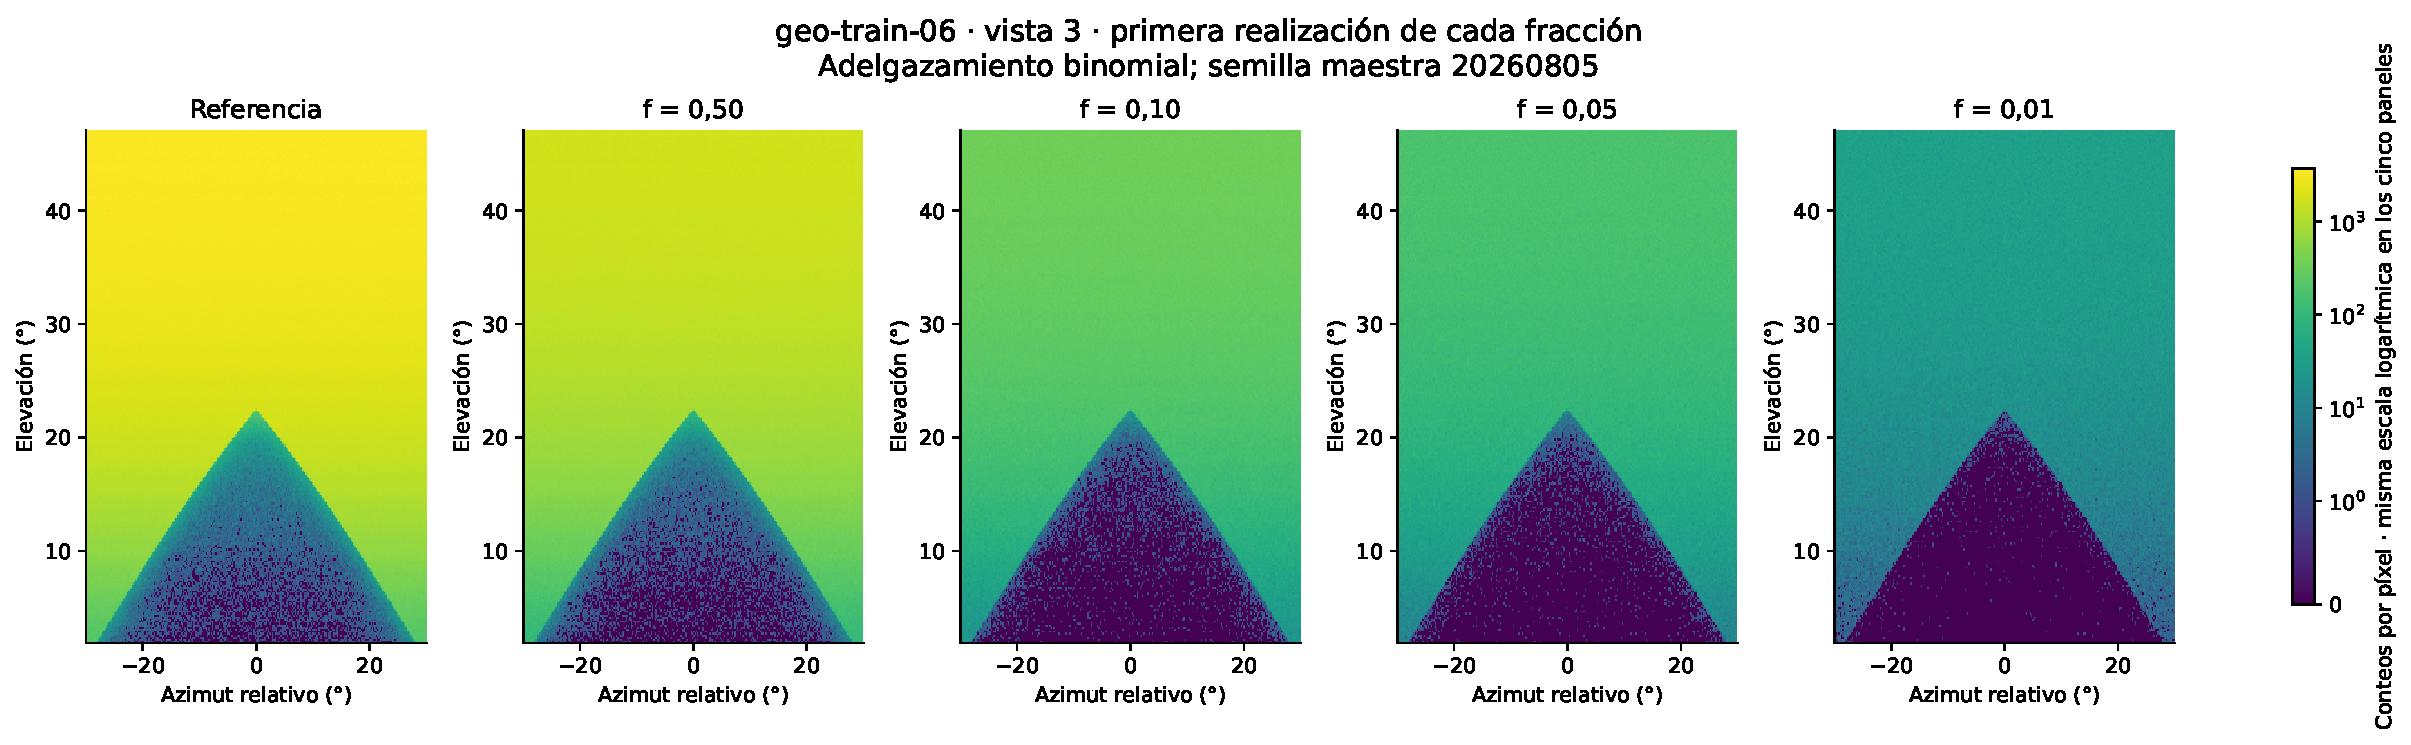
\includegraphics[width=\textwidth]{02-pares.pdf}
\caption{Referencia de \texttt{geo-train-06}, vista 3, y primera realización de cada fracción, con semilla maestra 20260805. Se muestran cuentas sin dividir por $f$. Los paneles comparten una referencia finita; no representan nuevas corridas independientes de transporte.}\label{fig:pares}
\end{figure}
\begin{figure}[p]\centering
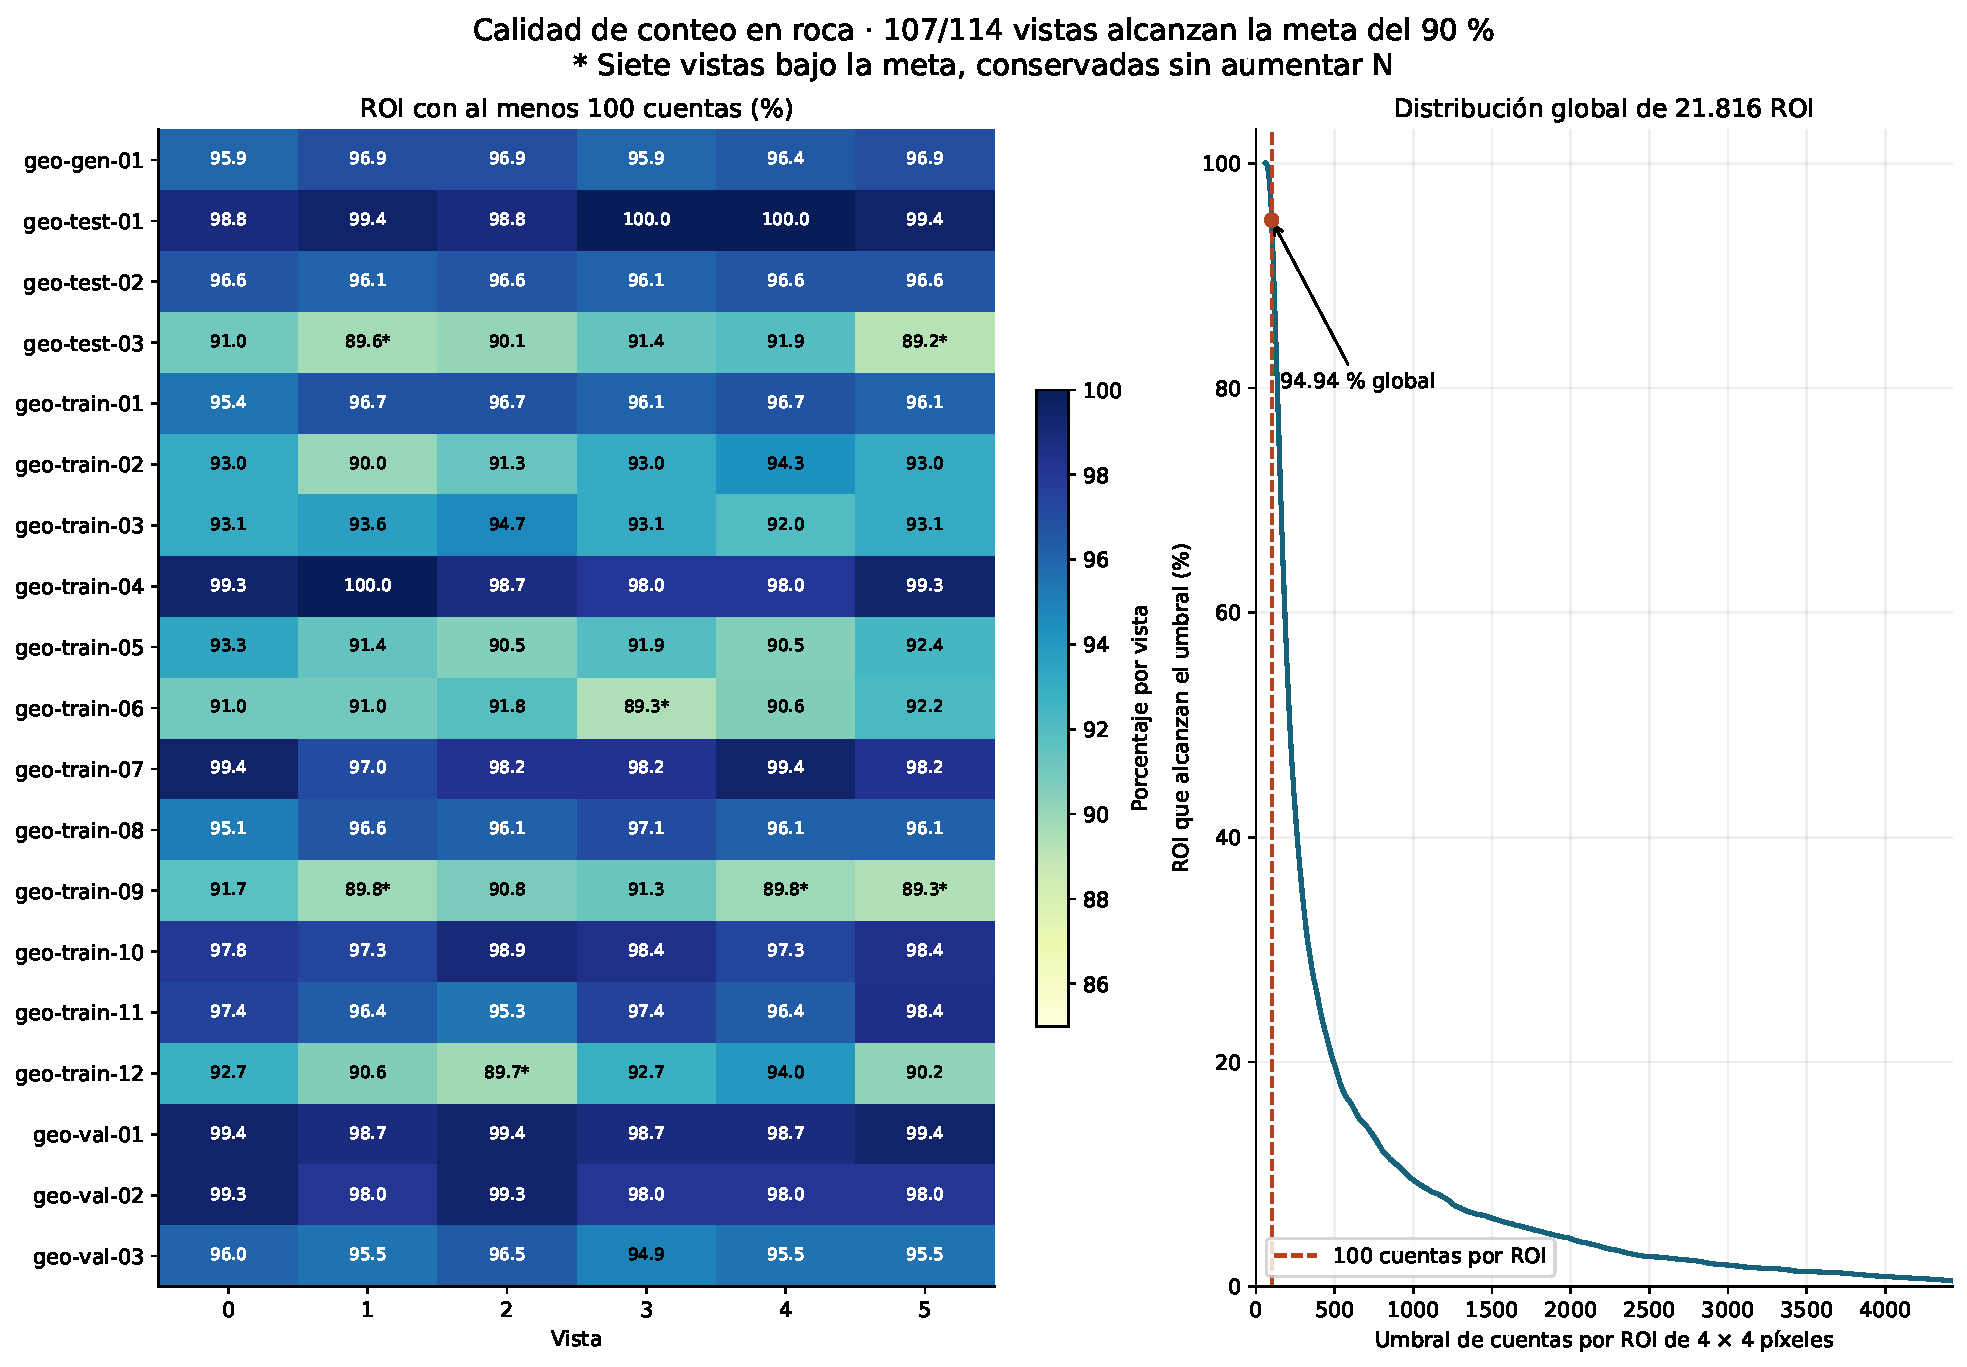
\includegraphics[width=\textwidth]{03-calidad-roca.pdf}
\caption{Porcentaje de ROI con al menos 100 cuentas por vista y distribución global de supervivencia de conteos. Se identifican las siete vistas bajo el $90\%$. La curva utiliza las 21.816 ROI; el eje horizontal se limita al percentil 99.5. El indicador global no sustituye la evaluación individual.}\label{fig:roca}
\end{figure}
\clearpage

\section{Discusión del alcance y las limitaciones}

La evidencia reunida permite sostener que se obtuvo un conjunto sintético organizado y reproducible bajo una receta explícita. Su valor reside en disponer de geometrías identificadas, vistas comparables, referencias con conteos conservados y realizaciones reducidas con una ley estadística conocida. La separación por geometría mantiene la unidad del escenario al reservar datos y evita mezclar en particiones distintas variantes derivadas de la misma referencia.

La representatividad es, sin embargo, acotada. Los conos y anomalías permiten estudiar respuestas de escenarios controlados, pero no incorporan por sí solos la complejidad topográfica, geológica y ambiental de un volcán concreto. La geometría reservada, que contiene un conducto y dos cavidades, aporta un caso adicional definido por el catálogo; una sola geometría de generalización no demuestra desempeño general frente a toda una población de volcanes. La justificación de representatividad desarrollada en este informe acota expresamente esta familia al propósito computacional del trabajo.

La fuente híbrida constituye otra condición del alcance. Los antecedentes de Guan y EcoMug sustentan componentes de la generación, pero no validan automáticamente su combinación, las extrapolaciones utilizadas o la inyección dirigida de esta implementación. Del mismo modo, el uso de Geant4 identifica una infraestructura física de transporte, mientras que la decisión de conservar solo primarios y la selección de llegada definen un observable específico. La verificación de archivos no reemplaza la evaluación de esas decisiones.

El contraste satisfactorio de bordes indica conformidad con una prueba de respuesta relativa a una fuente ideal sin transporte. No separa de manera única las contribuciones de aire, dispersión, migración angular o muestreo, ni acredita una aceptación instrumental calibrada. Esta delimitación es necesaria para interpretar los resultados favorables sin convertir una prueba concreta en una afirmación de validez física general.

En cuanto a la estadística, el presupuesto de 344 millones de primarios por vista produjo referencias de mayor conteo que sus realizaciones reducidas, pero no referencias exactas ni libres de ruido. Las siete vistas bajo la meta de roca muestran que un presupuesto común no garantiza la misma suficiencia en todas las regiones. Conservar estas diferencias evita presentar el conjunto como más uniforme o preciso de lo que indican sus datos. La covarianza de la ecuación~\eqref{eq:dependencia} advierte, además, que la cantidad de pares no es el tamaño de una muestra de simulaciones físicas independientes.

La trazabilidad lograda permite localizar la receta, repetir el posproceso y recuperar la copia distribuida. Las huellas verifican integridad respecto de una referencia concreta; no certifican por sí mismas corrección física, fecha de creación o permanencia futura del enlace. La revisión local no recompiló ni reejecutó Geant4 y no examinó todos los bloques crudos de SC3 a partir de la copia de Drive. Las conclusiones sobre ejecución se apoyan en los registros y productos documentados.

\section{Conclusión de cumplimiento del objetivo específico 1}

Se obtuvo un conjunto de imágenes sintéticas de muografía por transmisión para 19 escenarios volcánicos idealizados, observados desde seis vistas por escenario. La campaña produjo 114 referencias angulares de $256\times256$ píxeles a partir de 344 millones de primarios por vista. El adelgazamiento binomial con cuatro fracciones y veinte realizaciones por fracción permitió construir 9.120 pares de menor y mayor conteo, conservando su procedencia y su partición por geometría.

La identidad entre histogramas y matrices, la reproducción de los pares y la recuperación íntegra de la distribución respaldan el producto técnico correspondiente al OE1. Los controles de bordes cumplieron la tolerancia adoptada, mientras que la meta descriptiva de roca se alcanzó en 107 de las 114 vistas; las siete excepciones se conservaron y documentaron. De esta manera, el conjunto permite continuar el estudio computacional de imágenes con diferentes estadísticas dentro del alcance definido.

La conclusión se restringe a escenarios idealizados, conteos de primarios y exposición convencional. No implica mediciones de volcanes reales, equivalencia con un detector físico, una referencia sin ruido ni una reducción de tiempo de adquisición ya demostrada. La evidencia técnica y la justificación de representatividad quedan integradas en este informe. Por decisión expresa de la dirección, se da por cumplido y cerrado el OE1 dentro del alcance idealizado adoptado, conservando las siete excepciones de conteo y las limitaciones descritas. No queda una corrida de transporte requerida para este cierre. Esta decisión no acredita resultados de OE2 u OE3 ni sustituye la evaluación institucional del trabajo de grado.

\appendix
\section{Correspondencia con el objetivo y decisión de cierre}

El conjunto de imágenes sintéticas se acredita mediante 114 referencias; los distintos niveles de conteo mediante 9.120 pares; la generación Monte Carlo mediante la receta, los registros de SC3 y los productos de transporte; y la representatividad mediante la familia de mecanismos y configuraciones idealizadas justificada en este informe. La decisión de cierre conserva esa interpretación del objetivo, sin cambiar su enunciado ni introducir una validación instrumental no realizada.

Los criterios A-01 a A-08 y los pendientes P-01 a P-05 se consolidan en el registro de cierre del repositorio. Se conserva la atribución de la ejecución a los estudiantes y de la revisión a la dirección. La integración de este capítulo en la tesis completa y su presentación por los estudiantes son tareas editoriales y académicas del documento global; no constituyen nueva generación de datos pendiente del OE1.

La nomenclatura distingue primarios, cuentas, columna de masa y exposición convencional. Debe conservarse esta correspondencia al incorporar el texto a otros capítulos. El cierre del OE1 no declara finalizados los objetivos de aprendizaje profundo o de evaluación de reducción de adquisición.

\begin{thebibliography}{9}
\bibitem{agostinelli2003} S. Agostinelli y colaboradores. \emph{Geant4---a simulation toolkit}. Nuclear Instruments and Methods in Physics Research A, 506, 250--303, 2003. \href{https://geant4.web.cern.ch/about/publications.html}{Referencia oficial de Geant4}.
\bibitem{pagano2021} D. Pagano, G. Bonomi, A. Donzella, A. Zenoni, G. Zumerle y N. Zurlo. \emph{EcoMug: An Efficient COsmic MUon Generator for cosmic-ray muon applications}. Nuclear Instruments and Methods in Physics Research A, 1014, 165732, 2021. \href{https://dr4kan.github.io/EcoMug/index.html}{Documentación y referencia oficial}.
\bibitem{guan2015} M. Guan, M.-C. Chu, J. Cao, K.-B. Luk y C. Yang. \emph{A parametrization of the cosmic-ray muon flux at sea-level}. 2015. \href{https://arxiv.org/abs/1509.06176}{arXiv:1509.06176}.
\bibitem{receta} Proyecto muografia-documentada. \emph{Receta operativa del alcance idealizado}, versión preservada en 4529c49. \href{https://github.com/anlegogo/muografia-documentada/blob/4529c49/objetivo-1/contratos/receta-operativa-siete-actividades.json}{Configuración y huellas}. Los indicadores históricos de preparación no sustituyen los registros posteriores de ejecución.
\bibitem{estadistica} Proyecto muografia-documentada. \emph{Evaluación de bordes y control estadístico}, versión 4529c49. \href{https://github.com/anlegogo/muografia-documentada/blob/4529c49/herramientas/evaluar_bordes_angular.py}{Evaluador de bordes} y \href{https://github.com/anlegogo/muografia-documentada/blob/4529c49/herramientas/estadistica_control_angular.py}{intervalos y criterio}.
\bibitem{campana} Proyecto muografia-documentada. \emph{Revisión de campaña e037d09}, 3 de octubre de 2026. \href{https://github.com/anlegogo/muografia-documentada/blob/4529c49/objetivo-1/REVISION_CAMPANA_E037D09.md}{Registros de ejecución y límites de revisión}.
\bibitem{datos} Proyecto muografia-documentada. \emph{Revisión de datos f395570}, 3 de octubre de 2026. \href{https://github.com/anlegogo/muografia-documentada/blob/4529c49/objetivo-1/REVISION_DATOS_F395570.md}{Reproducción de referencias y pares}. \href{https://github.com/anlegogo/muografia-documentada/blob/4529c49/herramientas/empaquetar_angular_v1.py}{Esquema de adelgazamiento y semillas}.
\bibitem{drive} Proyecto muografia-documentada. \emph{Revisión independiente de la distribución en Drive}, 3 de octubre de 2026, commit 4529c49. \href{https://github.com/anlegogo/muografia-documentada/blob/4529c49/objetivo-1/REVISION_DISTRIBUCION_DRIVE.md}{Procedimiento, resultados e inventarios}.
\end{thebibliography}
\end{document}
